In this final section there is the alloy model, the world generated and the proof of consistency.
The model mainly describes the relationships between the various Data4Help entities. It's mainly shown how:
\begin{itemize}
\item It's impossible that multiple data sources of the same user tracks the same parameter.
\item Requests with filters (not targeted at a single user's data, but at a group of users' data defined by that filters and anonymized) are accepted by the system only if the filters cover a wide enough group to guarantee privacy.
\item Each user of AutomatedSOS is monitored by the system and, if hearth beat is lower or higher than the threshold range, the user is signaled to be in danger.
\item Each user that want to enroll in a run is monitored on his position by Track4Run
\item Each Spectator of Track4Run can only watch ongoing run and only if in that run are involved runners which positions are tracked
\end{itemize}
Moreover the world generated has 2 projected signatures: DataSources and Int. The consistency between the threshold values is nonetheless valid, even if omitted for readability. The same reasoning applies for DataSources, their are omitted to keep the image readable.\\

\lstinputlisting[language=alloy]{../Alloy/alloyReview.als}
\subsection{World Generated}
\centering
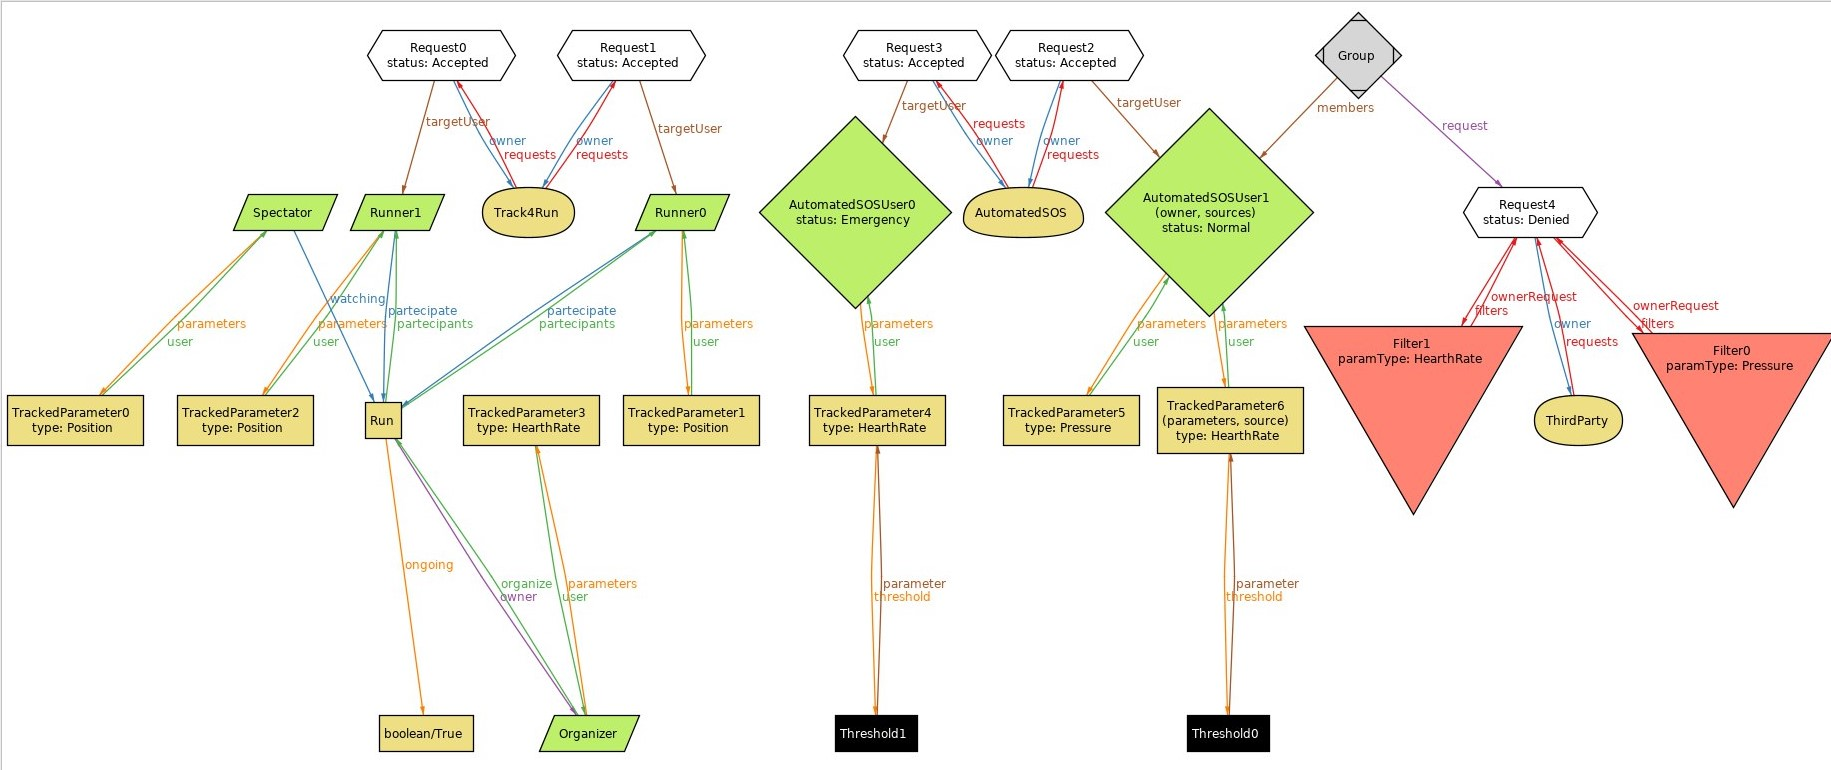
\includegraphics[angle=90, width =\textwidth, height=\textheight, keepaspectratio]{../Alloy/worldGenerated.jpg}\\
\subsection{Proof of consistency}
{
\centering
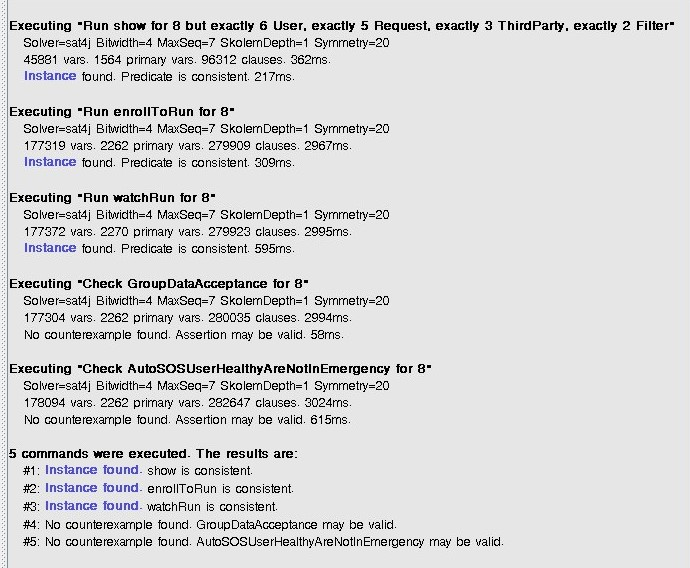
\includegraphics[width = 0.9\textwidth]{../Alloy/proofOfConcept.jpg}\\
}
